\section{Method}

Here we will discuss our implementation of cloud coverage analysis,
NDVI analysis, with use of beautiful flow charts. We should illustrate
the effectiveness of our analysis on test data.

\subsection{Thresholds}
Perhaps the most essential part of processing the EUMETSAT images is the ability
to differentiate between cloud and land. In order to do this, we rely on the
fact that clouds have a much higher reflectance than areas of land (notable
exceptions to this are snow, ice and salt pans). It follows that the
distribution of values for a single pixel over a large enough number of days
will be bimodal, the peak at the smaller value corresponding to land pixels and
the peak at the large value corresponding to cloudy pixels. The task is now one
of producing thresholds that reliably separate the two peaks. Otsu's method \cite{gonzalez2008} separates pixels into two groups, or \emph{classes}, by maximising the variance between these classes, making it an optimum method for thresholding \footnote{We have made use of \texttt{scipy}'s Otsu thresholding implementation.}. An example of Otsu thresholding at work is shown in Figure \ref{fig:otsu} for a random pixel.
\begin{center}
    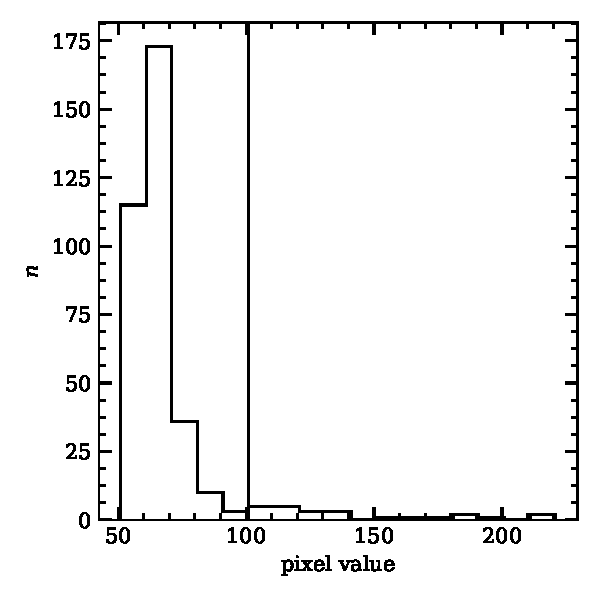
\includegraphics[width=\linewidth]{figures/otsu_bimodal.pdf}
    \captionof{figure}{The histogram of pixel values for a random pixel. Shown
      by the red line is the threshold calculated using Otsu's method -- it can
      be seen how well this method separates the two peaks.}
    \label{fig:otsu}
\end{center}
Now that we have the method for calculating the threshold of a single pixel all that remains is to apply it to the entire image, the process for doing so is detialed in Figure \ref{fig:thr_fc}.
% how do I put tikz in?
%% \begin{center}
%%   \documentclass{standalone}
\usepackage{tikz}
\usetikzlibrary{shapes,arrows,chains}
\begin{document}
% =================================================
% Set up a few colours
\colorlet{lcfree}{green}
\colorlet{lcnorm}{blue}
\colorlet{lccong}{red}
% -------------------------------------------------
% Set up a new layer for the debugging marks, and make sure it is on
% top
\pgfdeclarelayer{marx}
\pgfsetlayers{main,marx}
% A macro for marking coordinates (specific to the coordinate naming
% scheme used here). Swap the following 2 definitions to deactivate
% marks.
\providecommand{\cmark}[2][]{%
  \begin{pgfonlayer}{marx}
    \node [nmark] at (c#2#1) {#2};
  \end{pgfonlayer}{marx}
  } 
\providecommand{\cmark}[2][]{\relax} 
% -------------------------------------------------
% Start the picture
\begin{tikzpicture}[%
    >=triangle 60,              % Nice arrows; your taste may be different
    start chain=going below,    % General flow is top-to-bottom
    node distance=6mm and 60mm, % Global setup of box spacing
    every join/.style={norm},   % Default linetype for connecting boxes
    ]
% ------------------------------------------------- 
% A few box styles 
% <on chain> *and* <on grid> reduce the need for manual relative
% positioning of nodes
\tikzset{
  base/.style={draw, on chain, on grid, align=center, minimum height=4ex},
  proc/.style={base, rectangle, text width=8em},
  test/.style={base, diamond, aspect=2, text width=5em},
  term/.style={proc, rounded corners},
  % coord node style is used for placing corners of connecting lines
  coord/.style={coordinate, on chain, on grid, node distance=6mm and 25mm},
  % nmark node style is used for coordinate debugging marks
  nmark/.style={draw, cyan, circle, font={\sffamily\bfseries}},
  % -------------------------------------------------
  % Connector line styles for different parts of the diagram
  norm/.style={->, draw, lcnorm},
  free/.style={->, draw, lcfree},
  cong/.style={->, draw, lccong},
  it/.style={font={\small\itshape}}
}
% -------------------------------------------------
% Start by placing the nodes
\node [proc, densely dotted, it] (p0) {Calculating yearly thresholds};
% Use join to connect a node to the previous one 
\node [proc, join]      {Load full year of images $k$};
\node [proc, join]      {Slice image to region $(i,j)$};
\node [proc, join]      {Preallocate \texttt{threshold} as an array of size $(i,j)$};
\node [proc, join]      {Apply land mask};
\node [proc, join]      {Stack images in $(i,j,k)$ array};
\node [proc, join]      {\texttt{for} $x$ in the range $[0,i)$};
\node [proc, join]      {\texttt{for} $y$ in the range $[0,j)$};
\node [proc, join] (p1) {Select pixel slice $(x, y, :)$};
\node [proc, join] (p3) {Calculate \texttt{threshold}$(x,y)$ by Otsu's method};
\node [term, join]      {All threshold values calculated};

% No join for exits from test nodes - connections have more complex
% requirements
% We continue until all the blocks are positioned
% All the other connections come out of tests and need annotating
% First, the straight north-south connections. In each case, we first
% draw a path with a (consistently positioned) annotation node, then
% we draw the arrow itself.
%% \path (t1.south) to node [near start, xshift=1em] {yes} (p2);
%%   \draw [*->,lcnorm] (t1.south) -- (p2);

% -------------------------------------------------
\end{tikzpicture}
% =================================================

\end{document}

%%   \captionof{figure}{Flowchart for calculating threshold values.}
%%   \label{fig:thr_fc}
%% \end{center}


%% Local Variables:
%% fill-column: 80
%% End:
